\section{Foundry}
\label{sec:approach}

In this section, we present \FOUNDRY's workflow. Figure~\ref{fig:approach} overviews \FOUNDRY and how it is automated by \autoscalpel. Given an organs' entry point for the organ in the donor systems, its target implantation point in the product base, and a test suite that exercise the organ, it automatically: extracts an over-organ; constructs an organ-host compatibility layer; transforms the organ to be compatible with the context of its target sites in the product base; and implants it in the beneficiary's environment. All product derivation processes are performed in an iterative way where each organ is transplanted step-wise, and a new product is incrementally constructed as each organ is extracted and successfully transplanted. 

\begin{figure*}[t]
	\centering  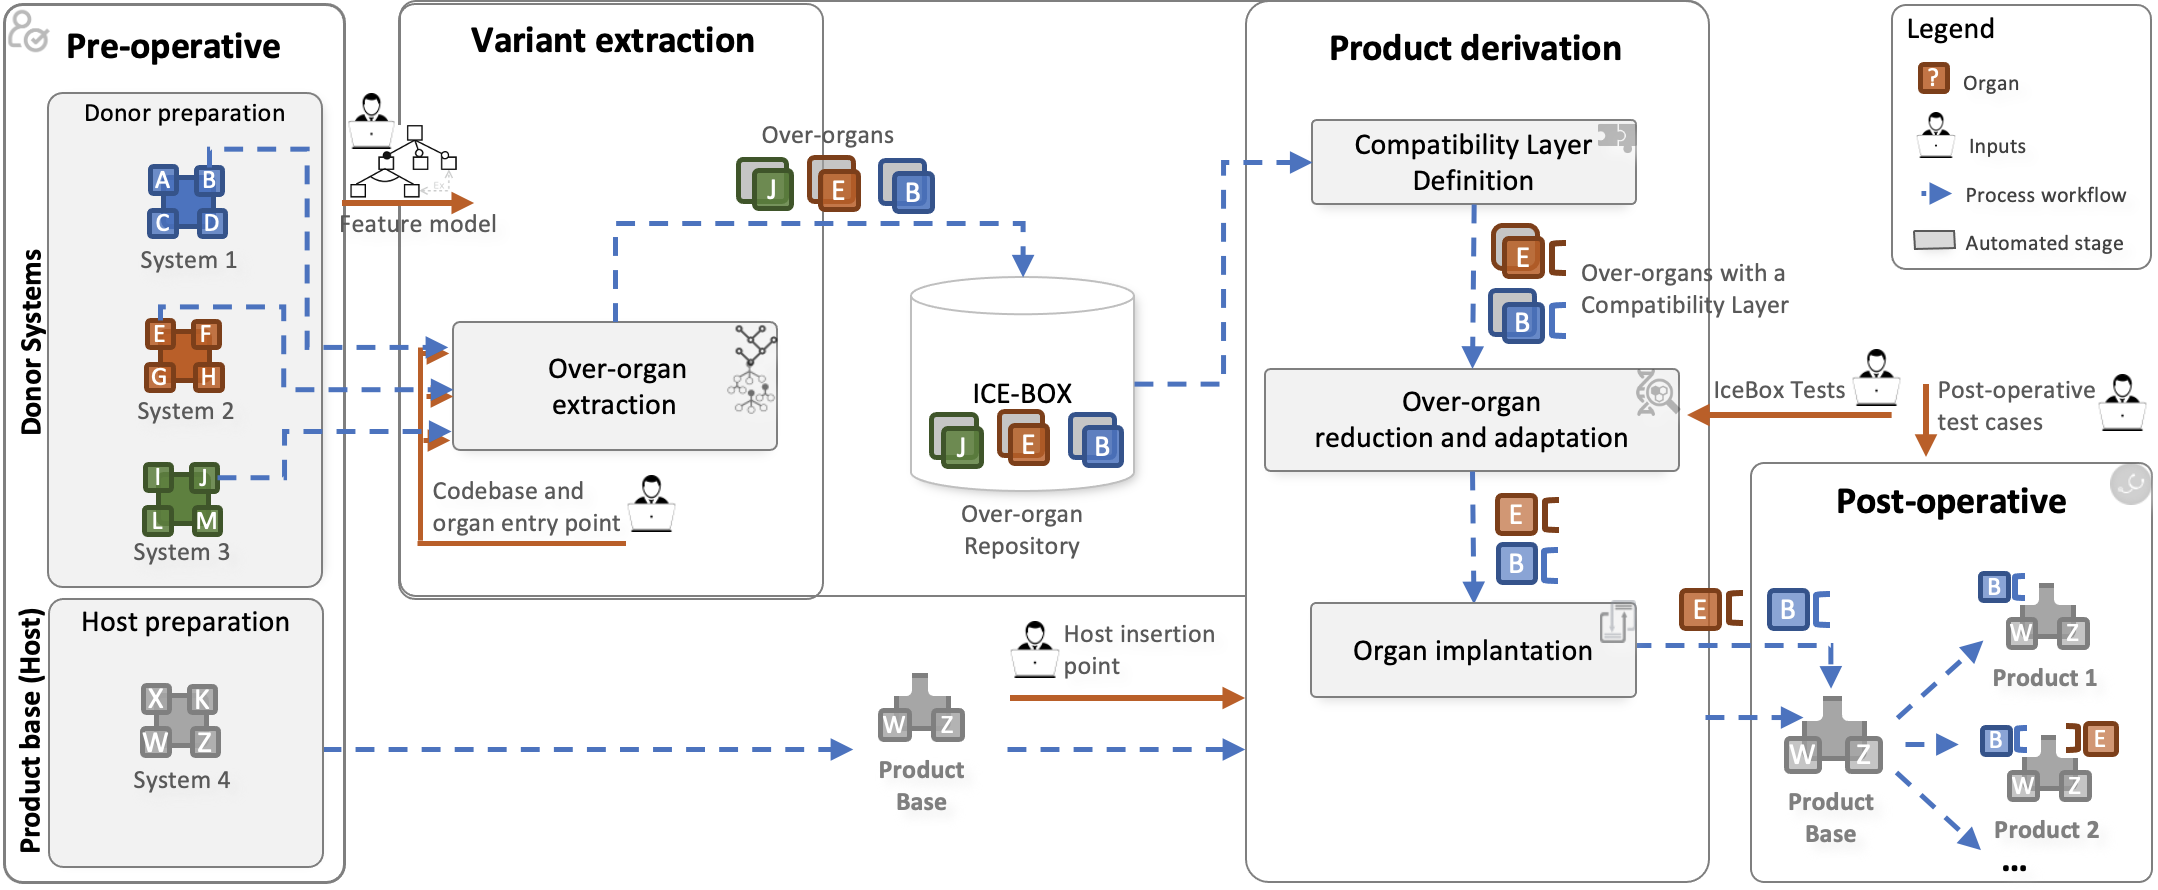
\includegraphics[width=18.5cm]{images/FOUNDRY3.png}
	\centering \caption{Overview of ST for generating product lines.}
	\label{fig:approach}
\end{figure*} 

Currently, \FOUNDRY is realized by \autoscalpel. The tool was implemented to generate product line representations from codebases written in C, however, the \FOUNDRY approach can be extend its scope to be used in the transplanting of features from codebases written in other languages. In this  section,  we provide details on the approach and how it is implemented by \autoscalpel

\subsection{Preoperative Stage} \pl{na figura tu colocou Pre-Operative}

As in medicine, our approach requires a \emph{preoperative} stage where donors and the host are prepared for the transplantation process and a \emph{postoperative} stage where the successful transplantation degree is evaluated. The preoperative stage defines a set of pre-transplantation tasks, responsible for the variability analysis process as well as the organ's test suite preparation. 

\subsubsection{Variability Analysis}

The preoperative stage starts with a variability analysis process in the donor candidates to discover features in existing products with the potential to compose the target product line. This task aims to create the variability model to express the valid combinations of features among the donor systems from which they will be extracted.  The variability model can be represented by using a feature model~\cite{Kang1990}.

Each feature representation in the feature model is annotated with 
its correspondent entry point (an organ entry point) in the donor codebase. An organ's entry point is a function in the donor systems that definitely belongs to the organ and defines correctly an execution environment expected for its initialization and provides the correct access to the organ's test suite. To determine the organ’s entry point, the user needs to provide the name of the function to \autoscalpel. 

\subsubsection{Donor Preparation}

Before starting the transplantation, the user selects a set of donor programs to provide features to the product line.It is spectated that one or more of those codebases can have annotations (e.g., code fragments guarded by \#ifdef C-preprocessor directives~\cite{Tartler2011})  commonly used to control code extensions related to features. Although useful for the donor program, such annotations, if transplanted, will generate dead code—fragments~\cite{Tartler2011} that will never be included in any valid feature selection. 

Using its \emph{Reconfigurator} and a textual list of preprocessor directives annotated with the prefix $\texttt{-D}$ provided by the user, \autoscalpel avoids these collateral effects by cleaning up unused directives and associated dead code from the donors. Thus, conditional directives belonging to the target organs are not transplanted to the host. This is done in a way that preserves as much of the source code structure belonging to the organ (indentation, spacing, number formats, etc.) as possible, to prevent future bugs. Figure~\ref{fig:reconfigurator} gives a example of a portion of code after \autoscalpel clean up unused directives.

\begin{figure}[t]
	\centering 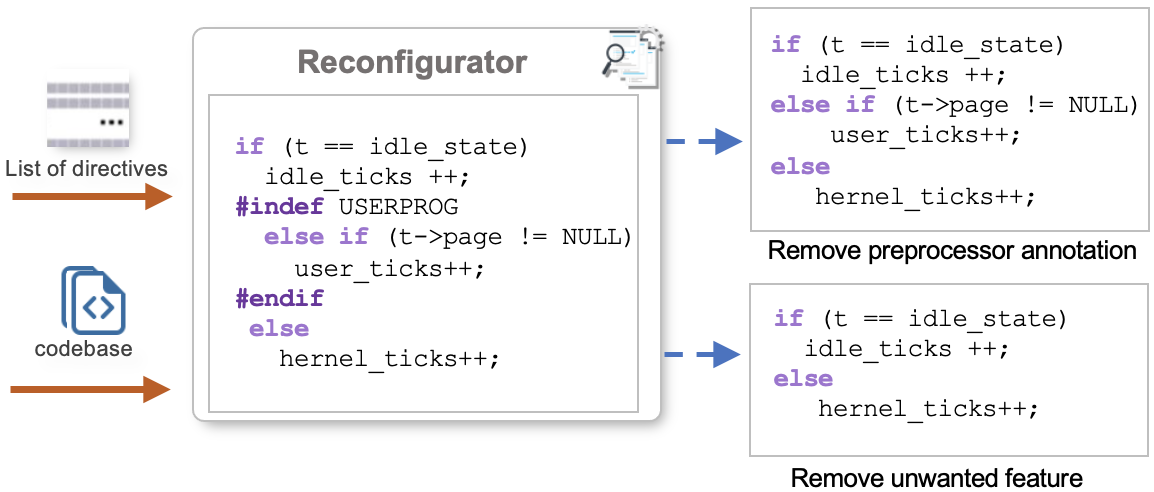
\includegraphics[width=9cm]{images/reconfigurator.png}
	\centering 
	\caption{The reconfigurator used to automated removal of preprocessor annotation from donor codebase and unwanted features from product base.}
	\label{fig:reconfigurator}
\end{figure} 

\subsubsection{Host preparation}

Still, during the pre-operative stage, the user has to select a product base from some existing system. If well-chosen, a product base can already provide a set of solutions so close to the target products that it can be used as a baseline for the assembly of the products to be generated. For example, a text edition program could provide a baseline for new programs for text translation,  presentation or rendering, since they could have a considerable number of common features among them.

The idea behind of product base is to take simultaneous advantage of commonality to reduce effort by transplanting only specific features required by each product variant. That is, while the product base provides commonalities (i.e. common features) to the target product line, the variabilities (i.e. variant features) are provided by the transplantation process, as illustrated by Figure~\ref{fig:product_for_transplantation}.

Case necessary the product base can be reduced to its basic form, keeping only mandatory or features relevant to the target product line. The reduction process consists of removal of all code that implements all features which will not be required to compose the product line. \autoscalpel's reconfigurator has been implemented to give support for the automatic feature removal from a codebase implemented using a mechanism like preprocessor directives. Such a mechanism allows the automatic identification and isolation of all fragments of code associated with a particular feature delimited such directives. 

\begin{figure}[t]
	\centering 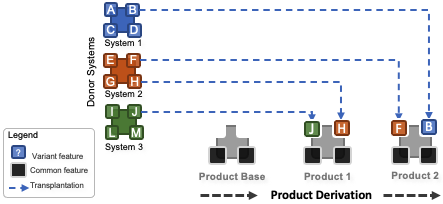
\includegraphics[width=\columnwidth]{images/product_for_transplantation.png}
	\centering 
	\caption{A product base used to generate different products.}
	\label{fig:product_for_transplantation}
\end{figure} 

To automate the feature removal process, \autoscalpel initially requires the user to provide as input a textual list of directives annotated with the prefix $\texttt{-U}$, corresponding to each feature to be removed. \autoscalpel then maps and searches selectively for pieces of code that implement features limited by such directives. Then, \autoscalpel removes all features source code from the product base while it keeps the source code structure belonging to the product base unchanged and ready to receive the transplanted organs.

In a removal scenario where the product base is implemented without a variability mechanism, additional attention is necessary to find and remove all portions of code that implement a target feature without compromising the codebase.

%%Note that a product base, once reduced, can be used multiple times as a base for new products. Although its preparation may require considerable effort for localising and removing all unnecessary code, it can be compensated with the benefits achieved through using the product base as a baseline to build other products belonging to the same or similar domain.

\subsection{Organ Test Suite Preparation}

For the transplantation process, the user also must supply test suites, called \emph{ice-box tests}~\cite{Barr2015}. They are used to guide GP in the search for extracted code modifications required to make the organ fully executable when implanted in the product base (see section~\ref{sec:organ_reduction}). The ice-box tests are implemented as \emph{in-situ}, a form of unit testing that starts from a valid program state rather than an arbitrary state~\cite{Barr2015}. Easily implementable, using the \emph{Check} unit testing framework for C~\cite{Check2019}, for instance, \emph{in-situ} unit testing allows us to leverage a single path to rigorously test whether the new functionality executes correctly in the host environment. 

Although ice-box tests can be quick to develop, it can be implemented using some existing test generation tools for C, or even adapted from donor’s unit tests to the host’s execution environment. 

\subsection{Over-organ Extraction}
Once the preoperative is stage done, and all inputs are prepared, we can start the automated organ extraction and transplantation process, using \autoscalpel. The code extracting process is a critical issue since it also involves identifying all semantically required code elements for the organ to be kept functional, even outside its original codebase. That way, the extraction of a target organ captures a considerable amount of code at different levels of granularity, from moving required files and libraries to entire functions and individual statements, both potentially not confined to a single file or library~\cite{Petrenko2009}.

We implemented a hybrid~\cite{Assuncao2017} process of extraction that uses a new kind of  GP, augmented by a form of dynamic observational slicing~\cite{Barr2015}, which we extended to compute slices from multiple files. The process of slicing discards those parts of the donor program that can be determined to have no effect upon the organ. Hence, it allows us to obtain an executable subset of program statements that preserves the original behaviour of the organ from its entry point in the donor program.

Figure~\ref{fig:over-organ_extraction} illustrates the slicing process. Technically, \autoscalpel builds call and caller graphs for each function implemented in the donor system. Then, it selects the call graphs corresponding to the organ's entry point. The organ's entry point is used as a starting point for automated organ slicing.

Using the observation-based slicing approach~\cite{Binkley:2014:OLP:2635868.2635893}, \autoscalpel reaches all functions from the organ's entry point. To find the over-organ, it slices forwards by isolating the donor's call graph edges that are particularly relevant to the organ under consideration. To compute a slice, it context-insensitively traverses the donor's call graph and transitively includes all the functions called by any function whose definition it reaches. The result is a set of slices that, when combined, produce an \emph{over-organ} that conservatively over-approximates the target organ~\cite{Barr2015}.

\begin{figure}[t]
	\centering 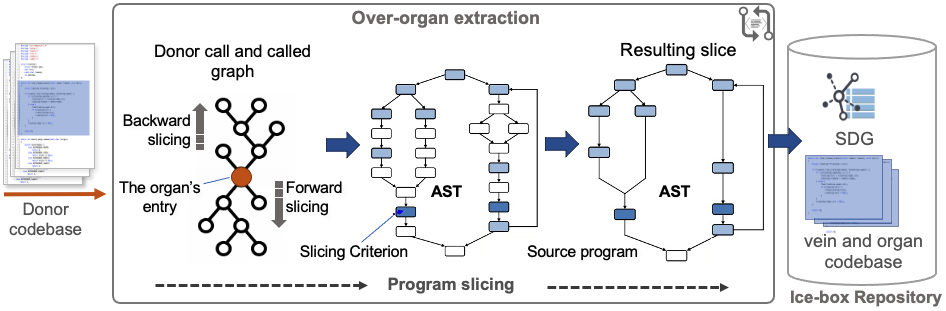
\includegraphics[width=\columnwidth]{images/over-organ_extraction2.png}
	\centering 
	\caption{Over-organ extraction process}
	\label{fig:over-organ_extraction}
\end{figure} 

The target organ implements the functionality to be transplanted; however, to be correctly initialized and executed, it requires an execution environment, called the vein~\cite{Barr2015} that correctly constructs the organ's parameters at its entry point. In the donor context, the execution environment is provided by one or more execution paths, that start at the donor's entry point (generally the function $\texttt{main}$) and ends at the organ's entry point. To compute a vein for an organ, \autoscalpel~slices backwards from the given organ's entry point traversing the call graph in reverse until it reaches the donor's entry point. Once it reaches the donor's entry point, \autoscalpel~prunes the slice to retain only the shortest path, under the assumption that all paths to the organ are equivalent. 

Once an over-organ is extracted, \autoscalpel~builds the donor's System Dependence Graphs (SDG)~\cite{Horwitz1988} which is used by GP to constrain its search space and to reject syntactically invalid offspring. Every function belonging to the call graph is represented as a dependency graph. Based on~\cite{Horwitz1988}, SDG includes data-dependence edges that represent transitive dependencies between function calls, in addition to the conventional direct-dependence edges. 

At the end of the extraction process, both organ and vein are kept in an IceBox repository to be, posteriorly, transplanted to the product base, deriving new product variants. 

\subsection{Compatibility Layer Definition}

Now we can start the derivation process when the target organ is then selected from Icebox to be pruned, adapted and implanted into the product base environment.

Harman et al.~\cite{Harman2013} proposed the construction of an interface between the transplant and the host into which candidate transplants can be initialized and evaluated. Following their proposal, we have introduced an \emph{organ-host converter}, a layer that works as a kind of organ-host interface responsible for providing access to the organ from the host.

The process of defining the interface is automated by using GP algorithm. It requires the correct mapping the parameters of the host-side implantation-point to the argument required by the organ's interface signature.Thus, the challenge for the GP algorithm is to efficiently find a binding between the host’s variable in scope at the implantation point inside the host to the organ’s interface parameters that correctly initialize an execution environment expected by the organ and provide the correct access by the organ’s tests. Some of these variables will need to be created and initialized during GP-refinement; others will use existing host variables. 

In practice, \autoscalpel inserts a call to the converter at the implantation point in the host. In the interface, \autoscalpel~ abstracts variable names so that GP can select a type-compatible binding. It selects different combinations of all valid statements and variables mapped from the organ's vein to initialize an execution environment that the organ expects before executing it. In the end, GP synthesizes a call to the extracted organ to execute it.

In addition to the benefits of encapsulation that this kind of organ-host interface provides, this converter also frees developers from the burden of writing the code to connect up and convert host data structures into organ parameters. For example, this converter may use a field reference to access a value the organ needs. Additionally, it will assist with testing and organ on-going maintenance.

\subsection{Over-organ Reduction and Adaptation}\label{sec:organ_reduction}

In this stage, GP is used to specialize the organ from the over-organ by decomposing it into an executable component that preserves the original behaviour of the feature at a given insertion point in the product base environment. The search space consists of all combinations of all valid statements and variables of the desired functionality in the donor and product base. 

Keeping the GP algorithm, implemented in~\cite{Barr2015}, our tool uses context insensitive slicing on the call graph of the donor program to construct a code map, with the key being the variables available in the vein, and the values being the variables in scope at the implantation point inside the host. Thus, the donor code statements are then available for \emph{crossover} and \emph{mutation} operations. 

By a mutation operation, a new version of a program (i.e., a new individual) is created by making several changes in the organ's interface and pruning the over-organ. Each such mutation operation is either an $\texttt{INSERT}$, $\texttt{REPLACE}$ and $\texttt{DELETE}$ of code into the individual at the level of statements. \autoscalpel~inlines all functions, then maps the over-organ's statements for which the GP needs to have access to an array; each array index uniquely identifies each statement. The chromosome of each individual has two parts: a host-to-organ map and a list of the indices in the over-organ that this individual includes. 

For each individual, GP uniformly selects a type compatible binding from the host's variables in scope at the implantation point to each of the organ's parameters. It then uniformly selects one statement from the over-organ, including its vein, and adds it to the individual. The GP system records which statements have been selected and favours statements that have not yet been selected.

In order to create individuals for the next generation, a crossover operation simply concatenates two individuals from the current population by appending one list to another. The first parent is chosen based on its fitness value while the other is chosen uniformly among those individuals from the breeding population, similar to the previous implementation inthe ~\cite{Petke2014}.

At each generation, \autoscalpel~selects the top 10\% most fit individuals and adds them into the new generation. We use tournament selection to select 60\% of the population for reproduction. Parents must be compilable; if the proportion of possible parents is less than 60\% of the population, GP generates new individuals and starts a new refinement loop. 

At each loop of GP-refinement, the candidate solution is then automatically evaluated using the ice-box tests. During ice-box testing, any calls the unit makes to its enclosing environment, like its host in autotransplantation, are compiled and executed. \autoscalpel~realizes a form of dynamic, observational slicing that removes redundant states from the vein while ensuring that the organ and its interface remain compilable and executable, and still correctly construct the parameters that the organ needs to retain the correct behaviour as defined by ice-box testing~\cite{Barr2015}. It loops over this state, modifying individuals to maximize coverage. At the end of the adaptation process, an organ that passes all the ice-box tests is selected uniformly and implanted into the product base in the implantation stage.

\subsection{Organ Implantation}

%\jp{I think this is an important point, as it emphasizes the difference between our approach and previous work, and thus should appear in the introduction.}
So far, the existing ST literature has discussed the transplantation of a single organ into a single codebase. Now, we consider how we implemented \autoscalpel to perform the transplant of multiple organs, including ones extracted from the same donor. In practice, an organ extracted from the same donor can be formed from code also belonging to other organs or already existing in the destination host, causing overlapping organs in the postoperative product base. 

Figure~\ref{fig:organs_connection_point} shows a real example of two call graphs from the same donor, GEdit text editor, sharing several functions. If we consider them as part of two unrelated organs, all common functions (highlighted by blue boxes) will be duplicated during their corresponding implantation processes.

\begin{figure}[t]
	\centering 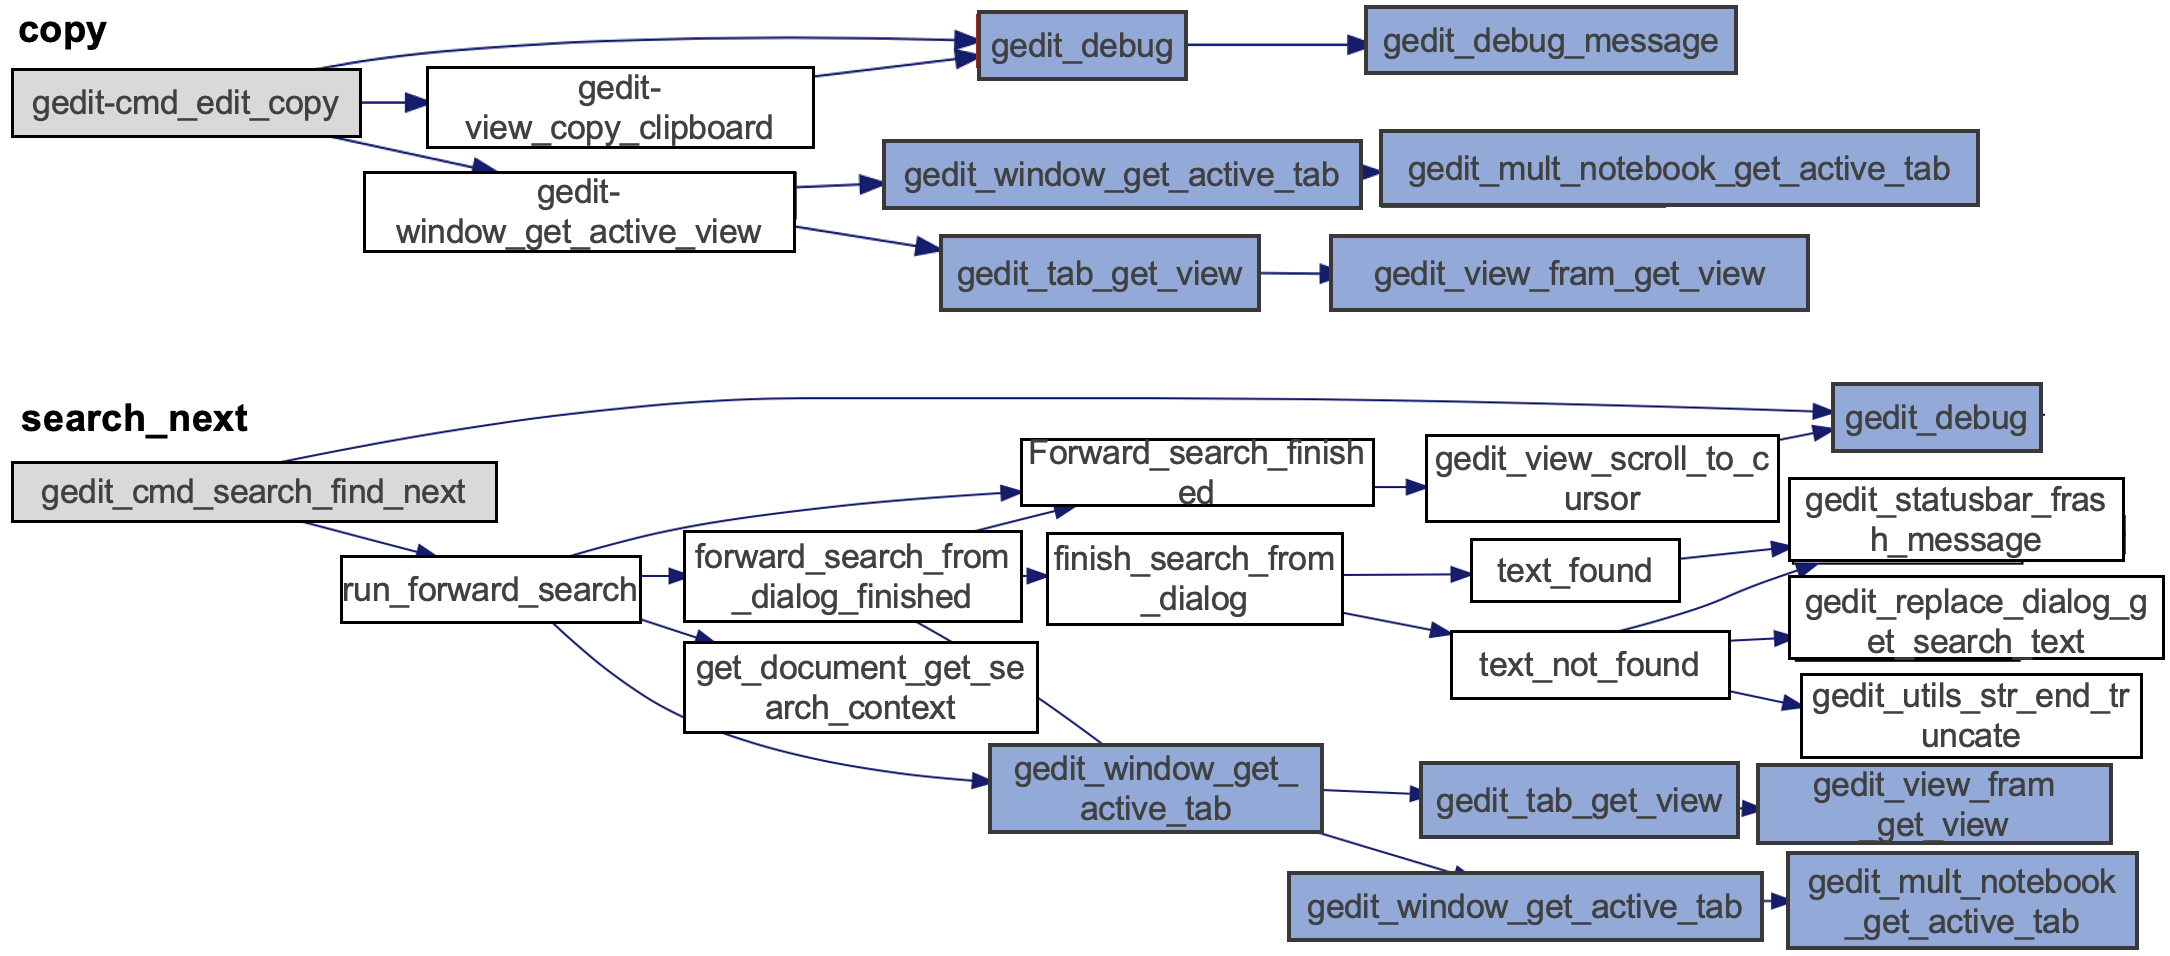
\includegraphics[width=\linewidth]{images/organs_dependency2.png}
	\caption{An example of connection points between the \emph{copy} and \emph{search\_next} organs. Highlighted with red boxes are functions belonging to both organs.}
%	\Description{The 1907 Franklin Model D roadster.}
	\label{fig:organs_connection_point}
\end{figure} 

Although the significant part of these overlaps is pruned from over-organ during GP-refinement, in the source code, one or more program elements within the boundaries of an organ depend on elements external to that organ, such as a function defined in one organ and called by another organ. In other words, organ dependencies are established by means of structural dependencies in the source code shared between elements of different organs~\cite{CafeoA2016}. When this happens, the \emph{organ collision} problem occurs that if it is not managed the transplantation process would add unwanted code duplication.

Thus, we need to do more than merely insert foreign code (self-contained) into the product base without any connections among the organs already transplanted. We need to augment the functionalities of the postoperative product base with new behaviour that replicates the software organ extracted from the donor without generating code duplication in a way that common parts of code may be shared among them.

In our approach, code elements (functions, directives, constants, declarations of several global variables and their definitions) already belonging to the beneficiary or to more than one organ are characterized as \emph{implicit connection points} since they can represent a connection or dependence points among two or more organs. That way, we need to identify these kinds of code elements and insert them one at a time, avoiding code duplication. However, hosts tend to have large input spaces into which \autoscalpel~inserts code. In this way, finding the implicit connection points in the host can be difficult. For instance, functions can have the same namespace but not be identical. Thus, it is necessary to check whether a specific code element is already present in the host, considering not only its namespace but its structure and context at a fine level of granularity to make sure that two portions of code are "clones".

We augmented \autoscalpel with a \emph{code clone detector}, based on NiCad~\cite{Roy2009}.  This clone detector finds exact clones over arbitrary program fragments in the organ and host source code by using Abstract Syntax Trees (AST). Thus, we exploit the benefits of \emph{Program differencing}~\cite{Kernighan1983} technique and TXL~\cite{Cordy2006} to identify and compare potential syntactic code duplication using text-line and ASTs comparison~\cite{Roy2009}

Figure~\ref{fig:code_clone_analysis} illustrates our solution to avoid the organ collision problem. To sum up, the clone detector checks if a specific code element is already present in the beneficiary's environment. Then, the code element is entirely \emph{grafted}, \emph{discarded}, or \emph{merged}. In this last case, \autoscalpel introduces additional line breaks such that potential variances within statements and other structures can be accurately inserted by using sub-abstract tree comparison. 

\begin{figure}[t]
	\centering 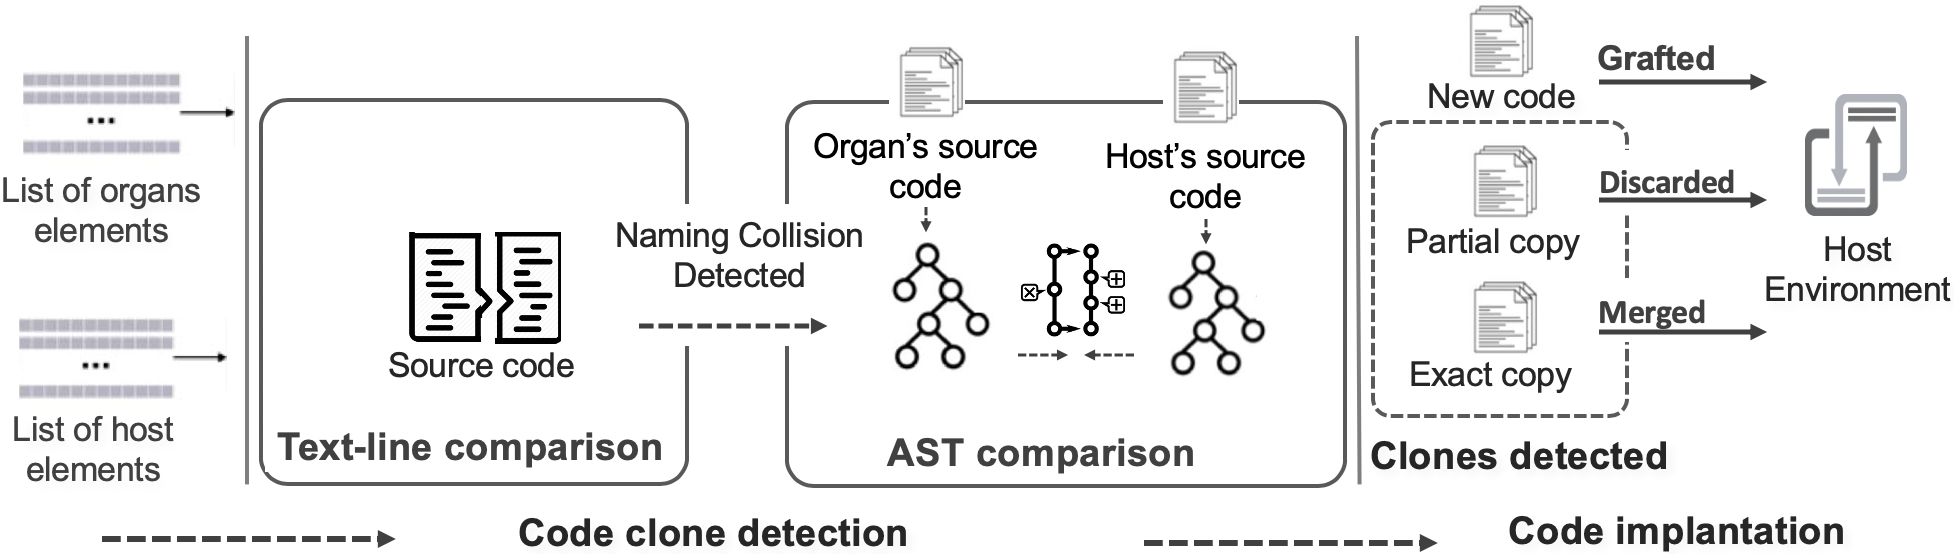
\includegraphics[width=\linewidth]{images/code_clone_analysis.png}
	\caption{Code clone resolution. }
	\label{fig:code_clone_analysis}
\end{figure} 

\subsection{Postoperative Stage} \label{ch:postoperative}

As in medicine, \FOUNDRY requires checking the side-effects of the transplantation operation. For this, we have to perform regression and acceptance testing. 

\FOUNDRY's last stage, its postoperative stage, introduces three validation steps, as outlined in Figure~\ref{fig:postoperative_tests}. Extending the validation process proposed in~\cite{Harman2013, Barr2015}, we highlight the three test suites that \FOUNDRY uses to evaluate the quality of a transplant:  Regression, Regression++, and/or Acceptance.

\FOUNDRY uses the product base's regression tests to check if the transplant does not disrupt the product base's behaviour. Some successful transplants add new functionality to the product base itself;  when that happens, the product base's \emph{regression} test suite must be updated with \emph{regression++} and  \emph{acceptance} tests from each such transplanted organ.

The  host's regression test suite is also manually augmented. Given the transplantation process introduces foreign code into the product base, it is unreasonable to expect its pre-existing test suite to continue to achieve high statement coverage. Hence, to achieve higher coverage, it can be necessary to add new tests to the host's existing test suite by creating regression++; %repetition: , an augmented regression test suite.

An \emph{acceptance} test suite for the postoperative product, manually updated to test the current transplanted functionality at the system level. It checks if the transplanted organ implements the new desired behaviour correctly. 

\begin{figure}[t]
	\centering 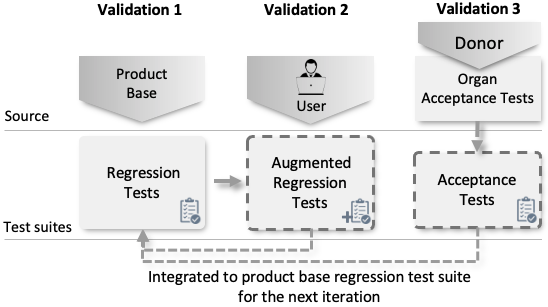
\includegraphics[width=7cm]{images/postoperative_tests2.png}
	\caption{Three validation steps; the dashed boxes are test cases added into the host regression test suite after each transplant iterations.}
	\label{fig:postoperative_tests}
\end{figure} 

Once \autoscalpel has successfully transplanted an organ into the product base, and the result has passed all postoperative validation steps, we incorporate the regression++ and acceptance tests into the host existing regression test suite for use in the next transplantation.

After this stage, new iterations of organ transplantation can be performed; thus, in a stepwise and incremental way, new products are derived as organs are transplanted. This process continues until all organs candidates have been transplanted, and the target product is derived. 
